\documentclass[11pt]{article}

% ------
% LAYOUT
% ------
\textwidth 165mm %
\textheight 230mm %
\oddsidemargin 0mm %
\evensidemargin 0mm %
\topmargin -15mm %
\parindent= 10mm

\usepackage[dvips]{graphicx}
\usepackage{multirow,multicol}
\usepackage[table]{xcolor}

\usepackage{amssymb}
\usepackage{amsfonts}
\usepackage{amsthm}
\usepackage{amsmath}

\usepackage{subfigure}
\usepackage{minted}

\graphicspath{{./pix/}} % put all your figures here.

\begin{document}
\begin{center}
\Large{\textbf{ECE 595: Homework 6}}

Yi Qiao, Class ID 187

(Spring 2019)
\end{center}

\section*{Exercise 1: Hoeffding Inequality}
\subsection*{(a) probability of getting a head for coins $c_1$, $c_{rand}$ and $c_{min}$}
Since they are all fair coins,
$$\mathbb{P}(c_1=head)=\mathbb{P}(c_{rand}=head)=\mathbb{P}(c_{min}=head)=0.5$$
\subsection*{(b) python experiment}
\begin{figure}[h]
	\centering
	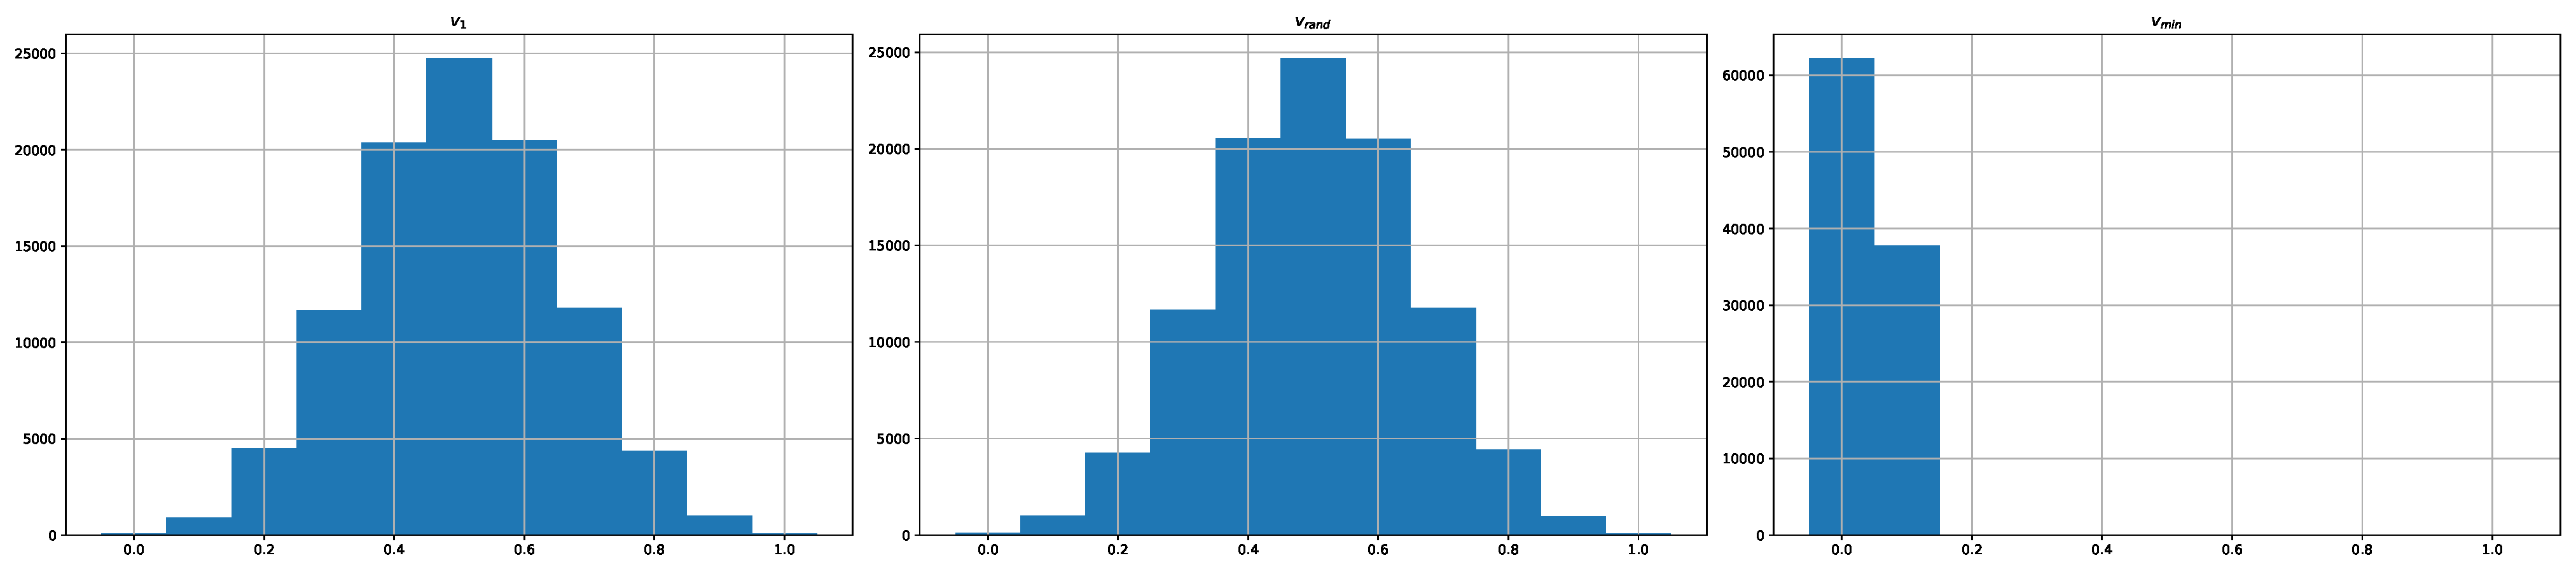
\includegraphics[width=\linewidth]{exercise1_b}
\end{figure}

The first two are binominal, while the third one is not.
\subsection*{(c) plots}
\begin{figure}[h]
	\centering
	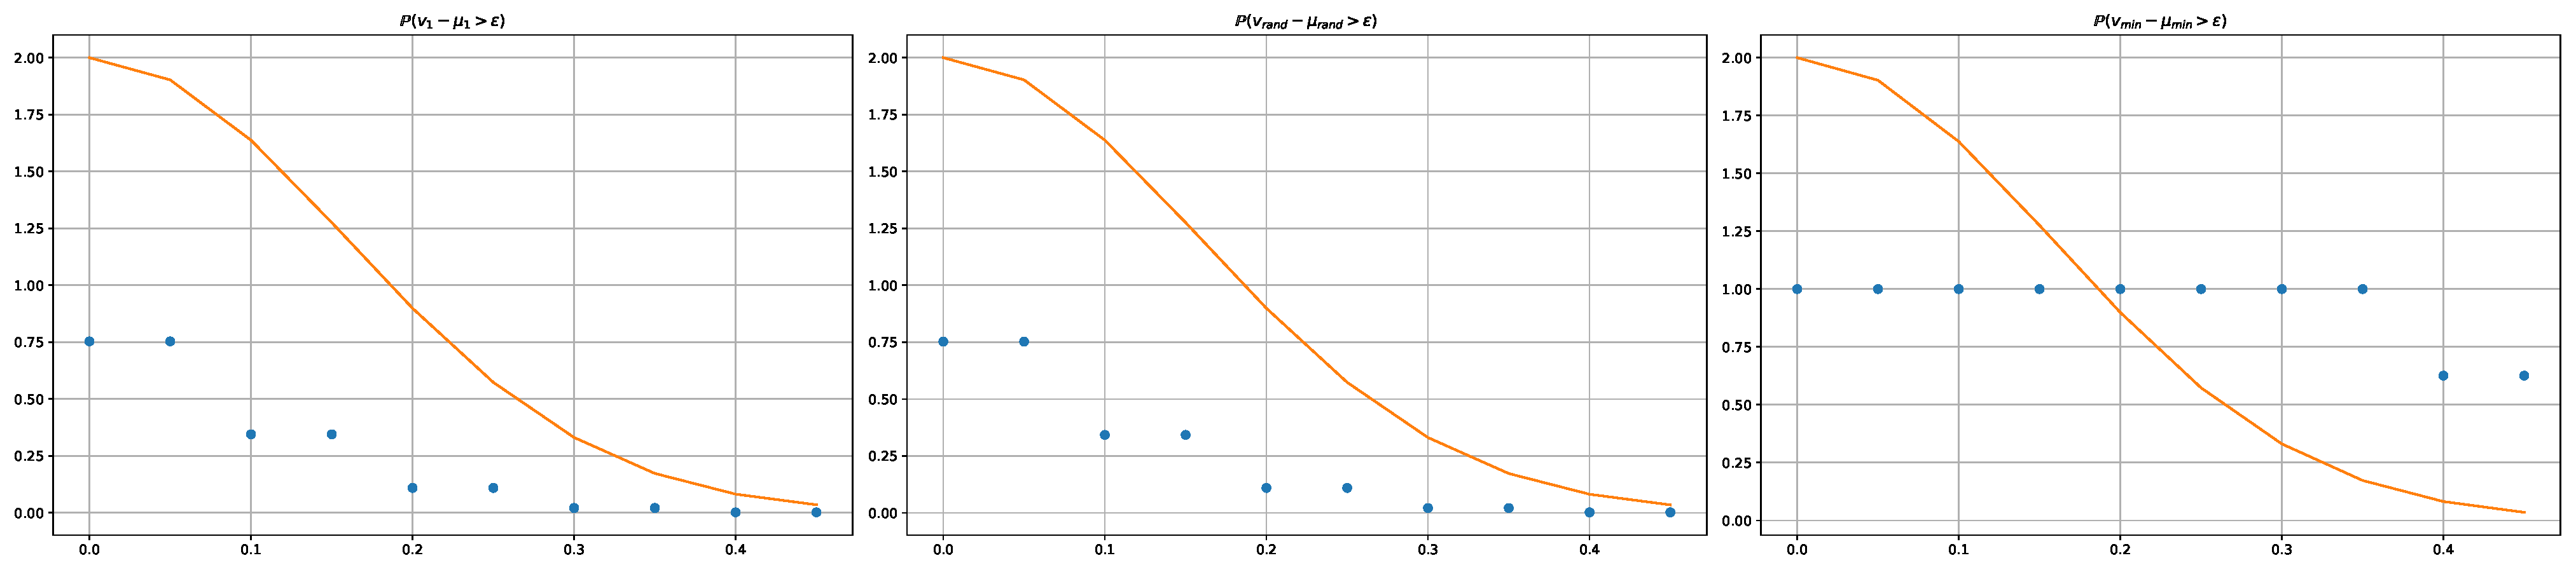
\includegraphics[width=\linewidth]{exercise1_c}
\end{figure}
\subsection*{(d)}
By observation, we can see that the first two obviously obey the Hoeffding's bound while the third one does not. This is because of its mean is different form its expectation, the expectation is around $0.38$ and the mean is $0.5$.
\subsection*{(e)}
This experiments states that, if we want to bound the error by Hoeffding, we have to make sure our data is i.i.d. and the expectation and mean are the same. 
\pagebreak
\section*{Exercise 2: VC Dimension}
\subsection*{(a) Compute the VC dimension}
\subsubsection*{(i)}	
\begin{equation}
\begin{split}
\mathcal{H}=&\{h:\mathbb{R}\rightarrow\{-1,+1\}|h(x)=+1,\forall x\in[a,\infty), a\in\mathbb{R}\} \cup \\
&\{h:\mathbb{R}\rightarrow\{-1,+1\}|h(x)=+1,\forall x\in(-\infty,a], a\in\mathbb{R}\}
\end{split}
\end{equation}
By inspection, the VC dimension of the above hypothesis set is 2. Since the hypothesis set is composed by two step functions that are symmetric to each other, they can shatter 2 points in 4 ways while obviously with one of the functions can get 3 combinations, $\{[+1,+1],[+1,-1],[-1,-1]\}$ by changing $a$, the other one will cover $\{[-1,-1],[-1,+1],[+1,+1]\}$, thus the union will be $\{[+1,+1],[+1,-1],[-1,+1],[-1,-1]\}$. While it is linear in a 1D space, it cannot shatter more than 2 points.

\subsubsection*{(ii)}
\begin{equation}
\begin{split}
\mathcal{H}=&\{h:\mathbb{R}\rightarrow\{-1,+1\}|h(x)=+1,\forall x\in[a,b], a,b\in\mathbb{R}\} \cup \\
&\{h:\mathbb{R}\rightarrow\{-1,+1\}|h(x)=-1,\forall x\in[a,b], a,b\in\mathbb{R}\}
\end{split}
\end{equation}
By inspection, the VC dimension of the above hypothesis set is 3. Similarly to the one above, The first hypothesis will cover $\{[-1,-1,-1],[-1,-1,+1],[-1,+1,+1],[+1,+1,+1],[+1,+1,-1],[+1,-1,-1]\}$, the second one will cover $\{[+1,+1,+1],[+1,+1,-1],[+1,-1,-1],[-1,-1,-1],[-1,-1,+1],[-1,+1,+1]\}$, the Union will cover all eight of them $\{[-1,-1,-1], ... ,[+1,+1,+1]\}$. While it is quadratic, it cannot shatter more than 3 points. 

\subsubsection*{(iii)}
\begin{equation}
\begin{split}
\mathcal{H}=&\left\{h:\mathbb{R}^d\rightarrow\{-1,+1\}|h(x)=+1,\forall x\ where \sqrt{\sum_{j=1}^{d} x_j^2}\le b, b\in\mathbb{R}\right\}
\end{split}
\end{equation}
By inspection, hypothesis function is a hyper ball. Thus, the VC dimension of the above hypothesis set is 1.

\subsection*{(b)}
\begin{equation}
\begin{split}
\mathcal{H}=&\left\{h_\alpha:\mathbb{R}\rightarrow\mathbb{R}|h_\alpha(x)=(-1)^{\lfloor \alpha x\rfloor},\alpha\in\mathbb{R}\right\}
\end{split}
\end{equation}
Even though the above hypothesis set has only one parameter, it is periodic, thus by tuning the period/frequency, you can match any number of data points you want by finding their GCD.
This hypothesis set has simply too large VC dimension, which is far beyond the model complexity. Thus, this will perform far worse than perceptron due to over-fitting.

\pagebreak
\section*{Exercise 3: Bias-Variance Trade-off}
\subsection*{(a)}
\begin{equation}
\begin{split}
\pmb{\theta}_\mathcal{D}=&\underset{\pmb{\theta}_h}{argmin}\ E_{aug}(h)\\
=&\underset{\pmb{\theta}_h}{argmin}\ E_{in}(h)+\frac{\lambda}{N}\pmb{\theta}^T_h\pmb{\theta}_h\\
=&\underset{\pmb{\theta}_h}{argmin}\ \frac{1}{N}\sum_{n=1}^{N}(\pmb{\theta}_h^T\pmb{x}_n-y_n)^2	+\frac{\lambda}{N}\pmb{\theta}^T_h\pmb{\theta}_h\\
=&\underset{\pmb{\theta}_h}{argmin}\ 
\left\lVert\begin{bmatrix}
\pmb{x}_1^T & 1\\
\pmb{x}_2^T & 1\\
\vdots & \vdots\\
\pmb{x}_N^T & 1\\
\end{bmatrix}
\pmb{\theta}_h - \pmb{y}\right\rVert^2_2
+\lambda\pmb{\theta}^T_h\pmb{\theta}_h\\
\end{split}
\end{equation}
substitute $\begin{bmatrix}
\pmb{x}_1^T & 1\\
\pmb{x}_2^T & 1\\
\vdots & \vdots\\
\pmb{x}_n^T & 1\\
\end{bmatrix}$
with $\pmb{A}$, we get
\begin{equation}
\begin{split}
\pmb{\theta}_\mathcal{D}=&\underset{\pmb{\theta}_h}{argmin}\ \left\lVert\pmb{A}\pmb{\theta}_h - \pmb{y}\right\rVert^2_2
+\lambda\pmb{\theta}^T_h\pmb{\theta}_h\\
\end{split}
\end{equation}
Taking the derivative, we can see
\begin{equation}
\begin{split}
\nabla_{\pmb{\theta}_h} &= 2\pmb{A}^T(\pmb{A\theta}_h-\pmb{y})+2\lambda\pmb{\theta}_h = 0\\
&(\pmb{A}^T\pmb{A}+\lambda\pmb{I})\pmb{\theta}_h = \pmb{A}^T\pmb{y}\\
&\pmb{\theta}_{\mathcal{D}}=\pmb{\theta}_h^* = (\pmb{A}^T\pmb{A}+\lambda\pmb{I})^{-1}\pmb{A}^T(\pmb{A}\pmb{\theta}_f+\pmb{\epsilon})
\end{split}
\end{equation}
\subsection*{(b)}
Continue from the last problem, expand what we already got,
\begin{equation}
\begin{split}
\pmb{\theta}_{\mathcal{D}}=& (\pmb{A}^T\pmb{A}+\lambda\pmb{I})^{-1}\pmb{A}^T(\pmb{A}\pmb{\theta}_f+\pmb{\epsilon})\\
=&(\pmb{A}^T\pmb{A}+\lambda\pmb{I})^{-1}\pmb{A}^T\pmb{A}\pmb{\theta}_f + (\pmb{A}^T\pmb{A}+\lambda\pmb{I})^{-1}\pmb{A}^T\pmb{\epsilon}\\
=&(\pmb{I}-\lambda\pmb{I}(\pmb{A}^T\pmb{A}+\lambda\pmb{I})^{-1})\pmb{\theta}_f + (\pmb{A}^T\pmb{A}+\lambda\pmb{I})^{-1}\pmb{A}^T\pmb{\epsilon}\\
=&\pmb{\theta}_f-\lambda(\pmb{A}^T\pmb{A}+\lambda\pmb{I})^{-1}\pmb{\theta}_f + (\pmb{A}^T\pmb{A}+\lambda\pmb{I})^{-1}\pmb{A}^T\pmb{\epsilon}\\
\end{split}
\end{equation}
\subsection*{(c)}
\subsubsection*{(i)}
\begin{equation}
\begin{split}
\bar{g}(\pmb{x}) &= \mathbb{E}_{\mathcal{D}}\left[h^{(\mathcal{D})}(\pmb{x})\right]=\mathbb{E}_{\mathcal{D}}\left[\pmb{\theta}_{\mathcal{D}}^T\pmb{x}\right]\\
&=\mathbb{E}_{\mathcal{D}}\left[\left(\pmb{\theta}_f-\lambda(\pmb{A}^T\pmb{A}+\lambda\pmb{I})^{-1}\pmb{\theta}_f + (\pmb{A}^T\pmb{A}+\lambda\pmb{I})^{-1}\pmb{A}^T\pmb{\epsilon}\right)^T\pmb{x}\right]\\
&=\pmb{\theta}_f^T\pmb{x}-\lambda\pmb{x}^T\mathbb{E}_{\pmb{A}}[(\pmb{A}^T\pmb{A}+\lambda\pmb{I})^{-1}]\pmb{\theta}_f+\pmb{x}^T\mathbb{E}_{\pmb{A}}[(\pmb{A}^T\pmb{A}+\lambda\pmb{I})^{-1}\pmb{A}^T]\mathbb{E}\left[\pmb{\epsilon}\right]\\
&=\pmb{\theta}_f^T\pmb{x}-\lambda\pmb{x}^T\mathbb{E}_{\pmb{A}}[(\pmb{A}^T\pmb{A}+\lambda\pmb{I})^{-1}]\pmb{\theta}_f
\end{split}
\end{equation}
\subsubsection*{(ii)}
\begin{equation}
\begin{split}
(\bar{g}(\pmb{x})-f(\pmb{x}))^2 =& ( \pmb{\theta}_f^T\pmb{x}-\lambda\pmb{x}^T\mathbb{E}_{\pmb{A}}[(\pmb{A}^T\pmb{A}+\lambda\pmb{I})^{-1}]\pmb{\theta}_f - \pmb{\theta}_f^T\pmb{x})^2\\
=&\lambda^2(\pmb{x}^T\mathbb{E}_{\pmb{A}}[(\pmb{A}^T\pmb{A}+\lambda\pmb{I})^{-1}]\pmb{\theta}_f)^T(\pmb{x}^T\mathbb{E}_{\pmb{A}}[(\pmb{A}^T\pmb{A}+\lambda\pmb{I})^{-1}]\pmb{\theta}_f)\\
=&\lambda^2(\pmb{\theta}_f^T\mathbb{E}_{\pmb{A}}[(\pmb{A}^T\pmb{A}+\lambda\pmb{I})^{-1}]^T\pmb{x}\pmb{x}^T\mathbb{E}_{\pmb{A}}[(\pmb{A}^T\pmb{A}+\lambda\pmb{I})^{-1}]\pmb{\theta}_f)\\
=&\lambda^2 trace(\pmb{x}\pmb{x}^T(\mathbb{E}_{\pmb{A}}[(\pmb{A}^T\pmb{A}+\lambda\pmb{I})^{-1}]\pmb{\theta}_f\pmb{\theta}_f^T\mathbb{E}_{\pmb{A}}[(\pmb{A}^T\pmb{A}+\lambda\pmb{I})^{-1}])
\end{split}
\end{equation}
\subsubsection*{(iii)}
Plug in $\pmb{A}^T\pmb{A}\approx N\pmb{I}$, we got 
\begin{equation}
\begin{split}
bias &= \mathbb{E}_{\mathcal{X}}[(\bar{g}(\pmb{x})-f(\pmb{x}))^2] \approx \lambda^2 trace(\mathbb{E}_{\mathcal{X}}[\pmb{x}\pmb{x}^T]((N+\lambda)\pmb{I})^{-1}\pmb{\theta}_f\pmb{\theta}_f^T((N+\lambda)\pmb{I})^{-1})]\\
&=\frac{\lambda^2}{(N+\lambda)^2}trace(\
\pmb{\theta}_f\pmb{\theta}_f^T)\\
&=\frac{\lambda^2}{(N+\lambda)^2}\
\pmb{\theta}_f^T\pmb{\theta}_f\\
&=\frac{\lambda^2}{(N+\lambda)^2}||\pmb{\theta}_f||^2_2
\end{split}
\end{equation}
\subsubsection*{(iv)}
\begin{equation}
\begin{split}
&\mathbb{E}_{\mathcal{D}}[(h^{(\mathcal{D})}(\pmb{x})-\bar{g}(\pmb{x}))^2] = \mathbb{E}_{\mathcal{D}}[(\pmb{\theta}_{\mathcal{D}}^T\pmb{x} - \pmb{\theta}_f^T\pmb{x}+\lambda\pmb{x}^T\mathbb{E}_{\pmb{A}}[(\pmb{A}^T\pmb{A}+\lambda\pmb{I})^{-1}]\pmb{\theta}_f)^2]\\
&=\mathbb{E}_{\mathcal{D}}[((\pmb{\theta}_f-\lambda(\pmb{A}^T\pmb{A}+\lambda\pmb{I})^{-1}\pmb{\theta}_f + (\pmb{A}^T\pmb{A}+\lambda\pmb{I})^{-1}\pmb{A}^T\pmb{\epsilon})^T\pmb{x} - \pmb{\theta}_f^T\pmb{x}+\lambda\pmb{x}^T\mathbb{E}_{\pmb{A}}[(\pmb{A}^T\pmb{A}+\lambda\pmb{I})^{-1}]\pmb{\theta}_f)^2]\\
&\approx\mathbb{E}_{\mathcal{D}}[(-\lambda\pmb{x}^T(N\pmb{I}+\lambda\pmb{I})^{-1}\pmb{\theta}_f + \pmb{x}^T(\pmb{A}^T\pmb{A}+\lambda\pmb{I})^{-1}\pmb{A}^T\pmb{\epsilon} +\lambda\pmb{x}^T(N\pmb{I}+\lambda\pmb{I})^{-1}\pmb{\theta}_f)^2]\\
&=\mathbb{E}_{\mathcal{D}}[(\pmb{x}^T(\pmb{A}^T\pmb{A}+\lambda\pmb{I})^{-1}\pmb{A}^T\pmb{\epsilon})^2]\\
&=\mathbb{E}_{\pmb{A}}[(\pmb{x}^T(\pmb{A}^T\pmb{A}+\lambda\pmb{I})^{-1}\pmb{A}^T)^2]\mathbb{E}_{\mathcal{\pmb{\epsilon}}}[\pmb{\epsilon}^2]\\
&=\sigma^2\mathbb{E}_{\pmb{A}}[(\pmb{x}^T(\pmb{A}^T\pmb{A}+\lambda\pmb{I})^{-1}\pmb{A}^T)^T(\pmb{x}^T(\pmb{A}^T\pmb{A}+\lambda\pmb{I})^{-1}\pmb{A}^T)]\\
&=\sigma^2\mathbb{E}_{\pmb{A}}[trace(\pmb{A}(\pmb{A}^T\pmb{A}+\lambda\pmb{I})^{-1}\pmb{x}\pmb{x}^T(\pmb{A}^T\pmb{A}+\lambda\pmb{I})^{-1}\pmb{A}^T)]\\
&=\sigma^2\mathbb{E}_{\pmb{A}}[trace(\pmb{x}\pmb{x}^T(\pmb{A}^T\pmb{A}+\lambda\pmb{I})^{-1}\pmb{A}^T\pmb{A}(\pmb{A}^T\pmb{A}+\lambda\pmb{I})^{-1})]
\end{split}
\end{equation}

\subsubsection*{(v)}
\begin{equation}
\begin{split}
var &= \mathbb{E}_{\mathcal{X}} [\mathbb{E}_{\mathcal{D}}[(h^{(\mathcal{D})}(\pmb{x})-\bar{g}(\pmb{x}))^2]]\\
&=\sigma^2\mathbb{E}_{\pmb{A}}[trace(\mathbb{E}_{\mathcal{X}}[\pmb{x}\pmb{x}^T](\pmb{A}^T\pmb{A}+\lambda\pmb{I})^{-1}\pmb{A}^T\pmb{A}(\pmb{A}^T\pmb{A}+\lambda\pmb{I})^{-1})]\\
&=\sigma^2\mathbb{E}_{\pmb{A}}[trace(\pmb{I}(\pmb{A}^T\pmb{A}+\lambda\pmb{I})^{-1}\pmb{A}^T\pmb{A}(\pmb{A}^T\pmb{A}+\lambda\pmb{I})^{-1})]\\
&=\sigma^2\mathbb{E}_{\pmb{A}}[trace((\pmb{A}^T\pmb{A})^{-1}\pmb{A}^T\pmb{A}(\pmb{A}^T\pmb{A}+\lambda\pmb{I})^{-1}\pmb{A}^T\pmb{A}(\pmb{A}^T\pmb{A}+\lambda\pmb{I})^{-1})]\\
&\approx\frac{\sigma^2}{N}\mathbb{E}_{\pmb{A}}[trace(\pmb{A}(\pmb{A}^T\pmb{A}+\lambda\pmb{I})^{-1}\pmb{A}^T\pmb{A}(\pmb{A}^T\pmb{A}+\lambda\pmb{I})^{-1})\pmb{A}^T]\\
&=\frac{\sigma^2}{N}\mathbb{E}_{\pmb{A}}[trace(H^2(\lambda))]
\end{split}
\end{equation}
\pagebreak
\section*{Code}
\inputminted[breaklines]{python}{./py/exercise1.py}
\end{document}


